%!TEX root = ../thesis.tex

\chapter{The $\tauhadvis$ reconstruction and identification at ATLAS}

\graphicspath{{1_MainChapters/Chap4_TauRec/figs}}
    This chapter describes the reconstruction (TauReco) and identification (TauID) of hadronically decaying tau leptons ($\tauhadvis$),
    largely based on the ``Reconstruction, Identification, and Calibration of hadronically decaying tau leptons 
    with the ATLAS detector for the LHC Run~3 and reprocessed Run~2 data''~\cite{ATL-PHYS-PUB-2022-044}. Over the 
    years, TauReco and TauID has been significantly improved, starting from 
    a cut-based approach adopted during early Run 1~\cite{ATL-PHYS-PUB-2010-001}, to a boosted decision tree (BDT)
    algorithm from the end of Run 1~\cite{PERF-2013-06}, and finally to a recurrent neural network (RNN) algorithm
    during Run 2 and Run 3~\cite{ATL-PHYS-PUB-2022-044}. In the future, TauID will be further improved by
    incorporating more advanced machine learning techniques such as graph neural networks (GNNs) and transformers.
    Early results from the GNN-based TauID have shown promising performance, with the potential to further enhance
    the signal-to-background separation in the $\tauhadvis$ identification.

\section{$\tauhadvis$ reconstruction}
    The candidates for $\tauhadvis$ are initially seeded by jets formed using the 
    anti-\(k_T\) algorithm, which has a radius parameter of $R = 0.4$. 
    The TopoClusters are calibrated using a local hadronic calibration (LC). 
    Jets that seed $\tauhadvis$ candidates must have \pt greater than 5 GeV and $|\eta| < 2.5$. 
    The \pT requirement is applied to the LC energy of the jet, prior to any JES corrections. 

    \subsection{Vertex association}
        During p-p collisions at the LHC, multiple simultaneous interactions occur, resulting in the reconstruction 
        of several interaction vertices. Typically, particles are assumed to originate from the primary vertex, 
        which is defined as the vertex with the highest sum of the squared transverse momenta of the associated 
        tracks (\(\sum p_T^2\)). However, since tau leptons decay away from the primary vertex, a dedicated 
        tau vertex association algorithm (TJVA) is used to identify the correct production vertex for each 
        $\tauhadvis$ candidate. This production vertex is then used for $\tauhadvis$
        reconstruction instead of the primary vertex.
        
        The tau production vertex is crucial for calculating quantities such as the impact parameter and determining 
        which tracks are associated with the $\tauhadvis$ candidate. Parameters of the associated 
        tracks are recalculated relative to the tau production vertex.
        
        For Run 3, the vertexing algorithm has been updated to handle the high pile-up environment, necessitating 
        a re-tuning of the TJVA. The method is based on the \pt fraction of a given vertex $f_{\pt}$:
        \[ f_{\pt} = \frac{\sum \pt (\text{tracks associated with the vertex})}{\sum \pt (\text{all tracks})} \]
        where all tracks within (\(\Delta R\)) of less than 0.2 from the seed jet are considered. The vertex 
        with the highest $f_{\pt}$ fraction is chosen as the tau production vertex and is used for determining 
        the $\tauhadvis$ direction, associating tracks, and building the coordinate system for calculating 
        identification variables.
        
        The efficiency of selecting the correct tau production vertex compared to the primary vertex is evaluated 
        as a function of the \tauhadvis \pt and the average number of simultaneous proton-proton 
        collisions ($\langle \mu \rangle$). The tau production vertex consistently shows better efficiency, 
        especially at low \pt.
        
        The $\tauhadvis$ four-momentum is calculated by first computing \(\eta\) and \(\phi\) of 
        the barycentre of the TopoClusters of the seed jet, calibrated at the LC scale, assuming a mass of zero 
        for each constituent. The four-momenta of all clusters in the region \(\Delta R < 0.2\) around the 
        barycentre are recalculated using the tau production vertex coordinate system and summed, providing 
        the momentum magnitude and direction of the $\tauhadvis$. Figure \ref{fig:tau_vtx_eff} shows the 
        efficiency to select the correct $\tau$ production vertex using TJVA or the default primary vertex
        in $\gamma^*\rightarrow\tau\tau$ events, as a function of $\langle \mu \rangle$, taken from~\cite{ATL-PHYS-PUB-2022-044}.
        \begin{figure}[htbp]
            \centering
            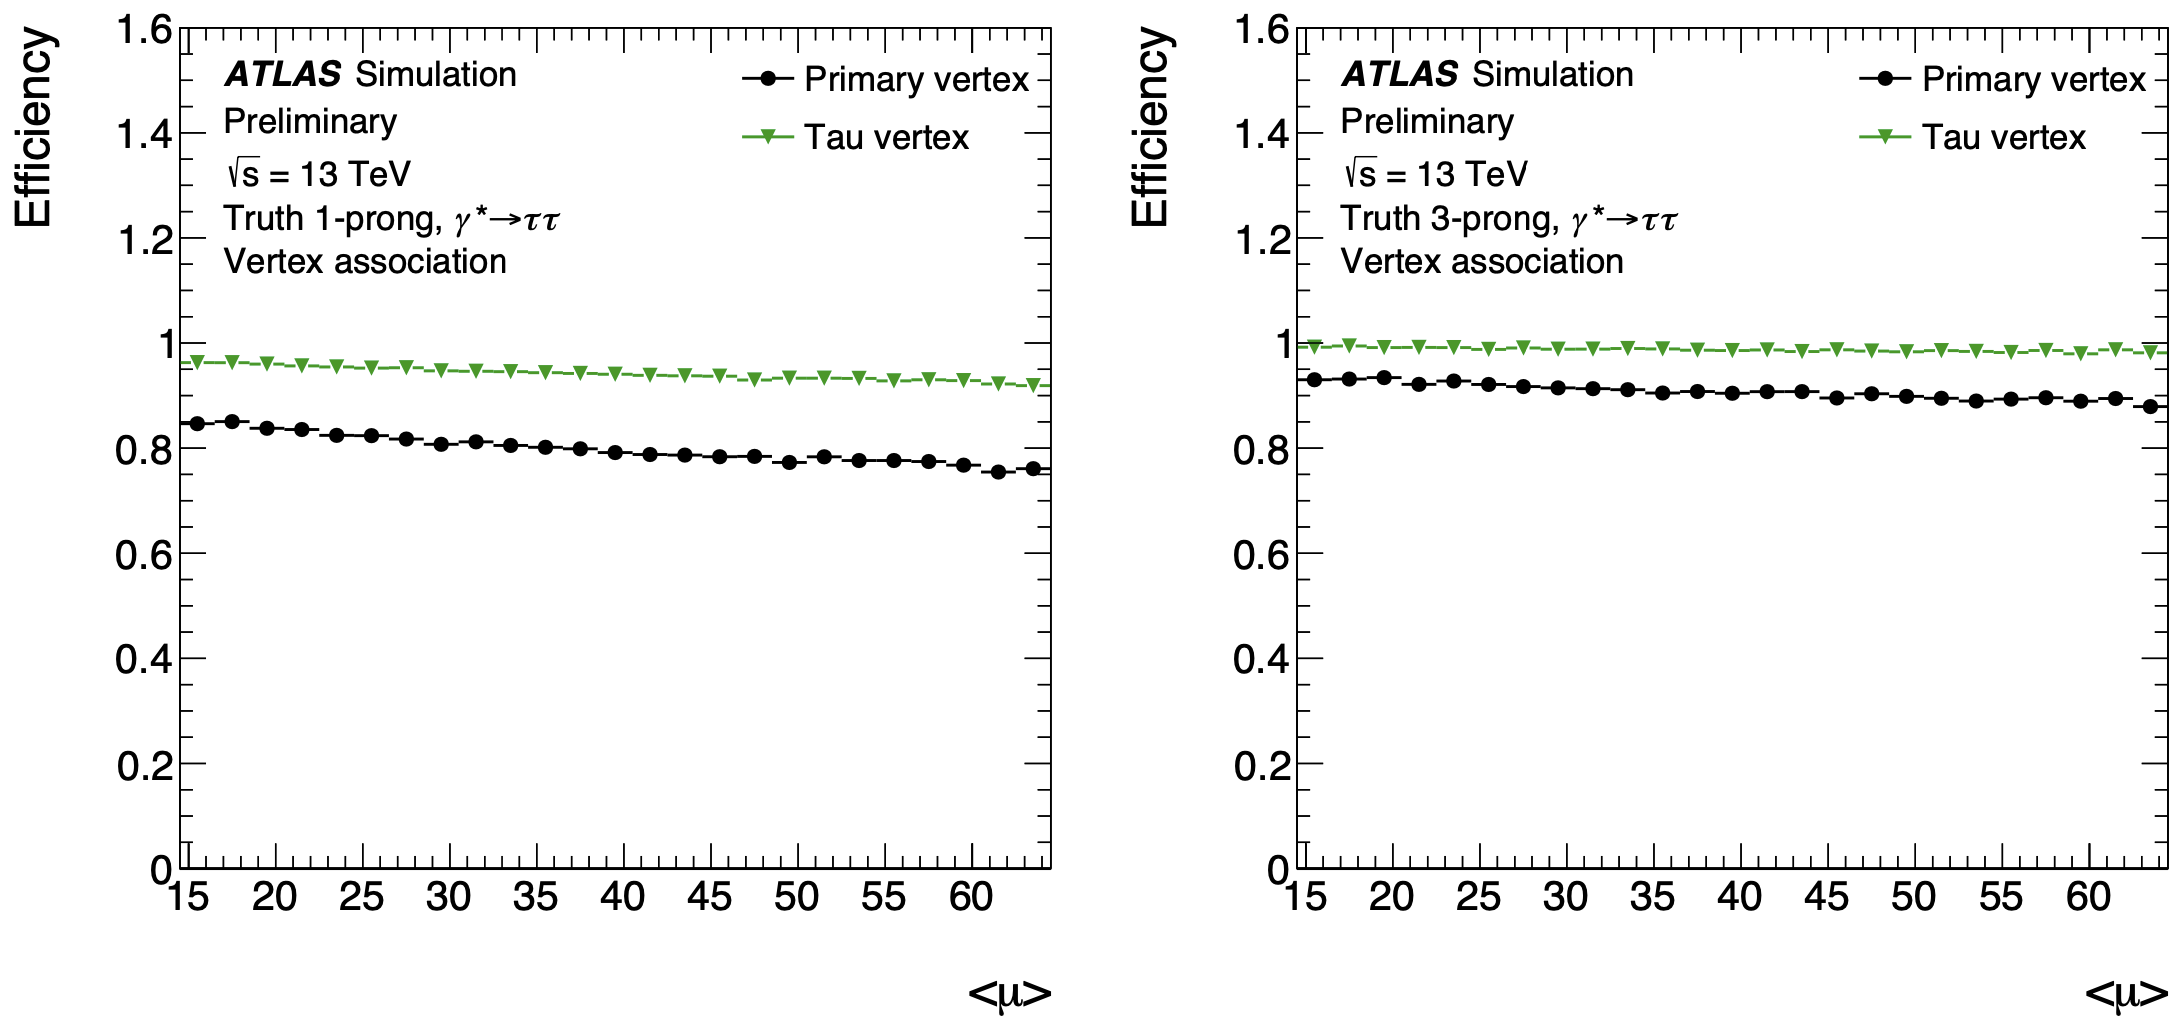
\includegraphics[width=0.9\textwidth]{vtx_tagging}
            \caption{
                Efficiency to select the correct $\tau$ production vertex using TJVA or the default primary vertex in $\gamma^*\rightarrow\tau\tau$ events, as a function of $\langle \mu \rangle$. 
                The left plot shows the efficiency for 1-prong $\tauhad$, while the right plot shows the efficiency for 3-prong $\tauhad$, taken from~\cite{ATL-PHYS-PUB-2022-044}.
            }
            \label{fig:tau_vtx_eff}
        \end{figure}
        
    \subsection {Track Association}
        Tracks are associated with the $\tauhadvis$ candidate if they are within a core region 
        (\(\Delta R < 0.25\)) around the $\tauhadvis$ direction and meet the following criteria:
        \begin{itemize}
            \item \pt greater than 1 GeV,
            \item at least two associated hits in the pixel layers of the inner detector,
            \item at least seven hits in total in the pixel and SCT layers.
        \end{itemize}
        Additionally, association requirements are imposed on the distance of closest approach of the track 
        to the tau production vertex in the transverse plane (\(|d_{0}^{\text{TJVA}}| < 1.0\) mm) and 
        longitudinally (\(|z_{0}^{\text{TJVA}} \sin \theta | < 1.5\) mm).
        Tracks in the region \(0.25 < \Delta R < 0.4\) are also associated with the $\tauhadvis$if either:
        \begin{itemize}
            \item they are matched to the \tauseed jet by a ghost-particle association technique, or
            \item the closest jet to the track in terms of \(\Delta R\) distance is the $\tauhadvis$ seeding jet.
        \end{itemize}
    
    \subsection {Track Classification}
        To correctly establish the charge and the number of charged decay products of a tau lepton, the tracks that are 
        associated with the tau decay need to be correctly distinguished from the other tracks associated with the \tauseed. 
        Using a track classifier, tracks that have passed the TJVA requirements are classified into four categories:
        \begin{itemize}
            \item tau tracks (TT): tracks originating from charged tau lepton decay products.
            \item conversion tracks (CT): tracks from electrons and positrons that are created from photon conversion in the detector.
            \item isolation tracks (IT): tracks likely originating from quark or gluon jets arising from the remnants of the hard scattering interactions.
            \item fake tracks (FT): tracks that do not belong to the previous categories, mainly misreconstructed tracks and pile-up tracks.
        \end{itemize}
        A novel approach for the tau lepton track classification using a recurrent neural network 
        (RNN)~\cite{schmidt2019recurrentneuralnetworksrnns} has been developed, 
        replacing the previous BDT-based method used during Run 2. RNNs are specifically chosen for their ability to use 
        bidirectional long short-term memory (BLSTM) cells, 
        allowing information to be back-propagated, exploiting 
        forward and backward correlations in sequences of tracks belonging to tau decays.
    
        % The RNN architecture includes three dense layers connected to the input (tracks of the $\tauhadvis$ candidate). 
        % Three BLSTM layers are configured between the dense layers. And one output layer was configured, comprising four nodes, each associated 
        % with a track classifier category. 
        The network is trained using Keras~\cite{chollet2015keras} and TensorFlow~\cite{tensorflow2015-whitepaper}, 
        applied to sequences of \pt-ordered tracks associated with 
        each $\tauhadvis$ candidate. The training data includes signal candidates from simulated \(\gamma^* \rightarrow \tau\tau\) 
        events and background candidates from dijet events, with each sample divided into subsets for training, validation, and performance evaluation. 
        Input variables for the RNN include kinematic, geometric, and detector hit distribution information for the tracks. 
        The primary measure to evaluate the performance of the track classifier are the reconstruction efficiency.
        The reconstruction efficiency is the efficiency to correctly classify 1- or 3-tracks originating from truth 1-prong and 3-prong \(\tau\) leptons.
        The reconstruction efficiency evaluated as a function of the $\tauhadvis$ $pT$ and $\langle \mu \rangle$ is shown in Figure \ref{fig:track_classification_eff}.
        \begin{figure}[htbp]
            \centering
            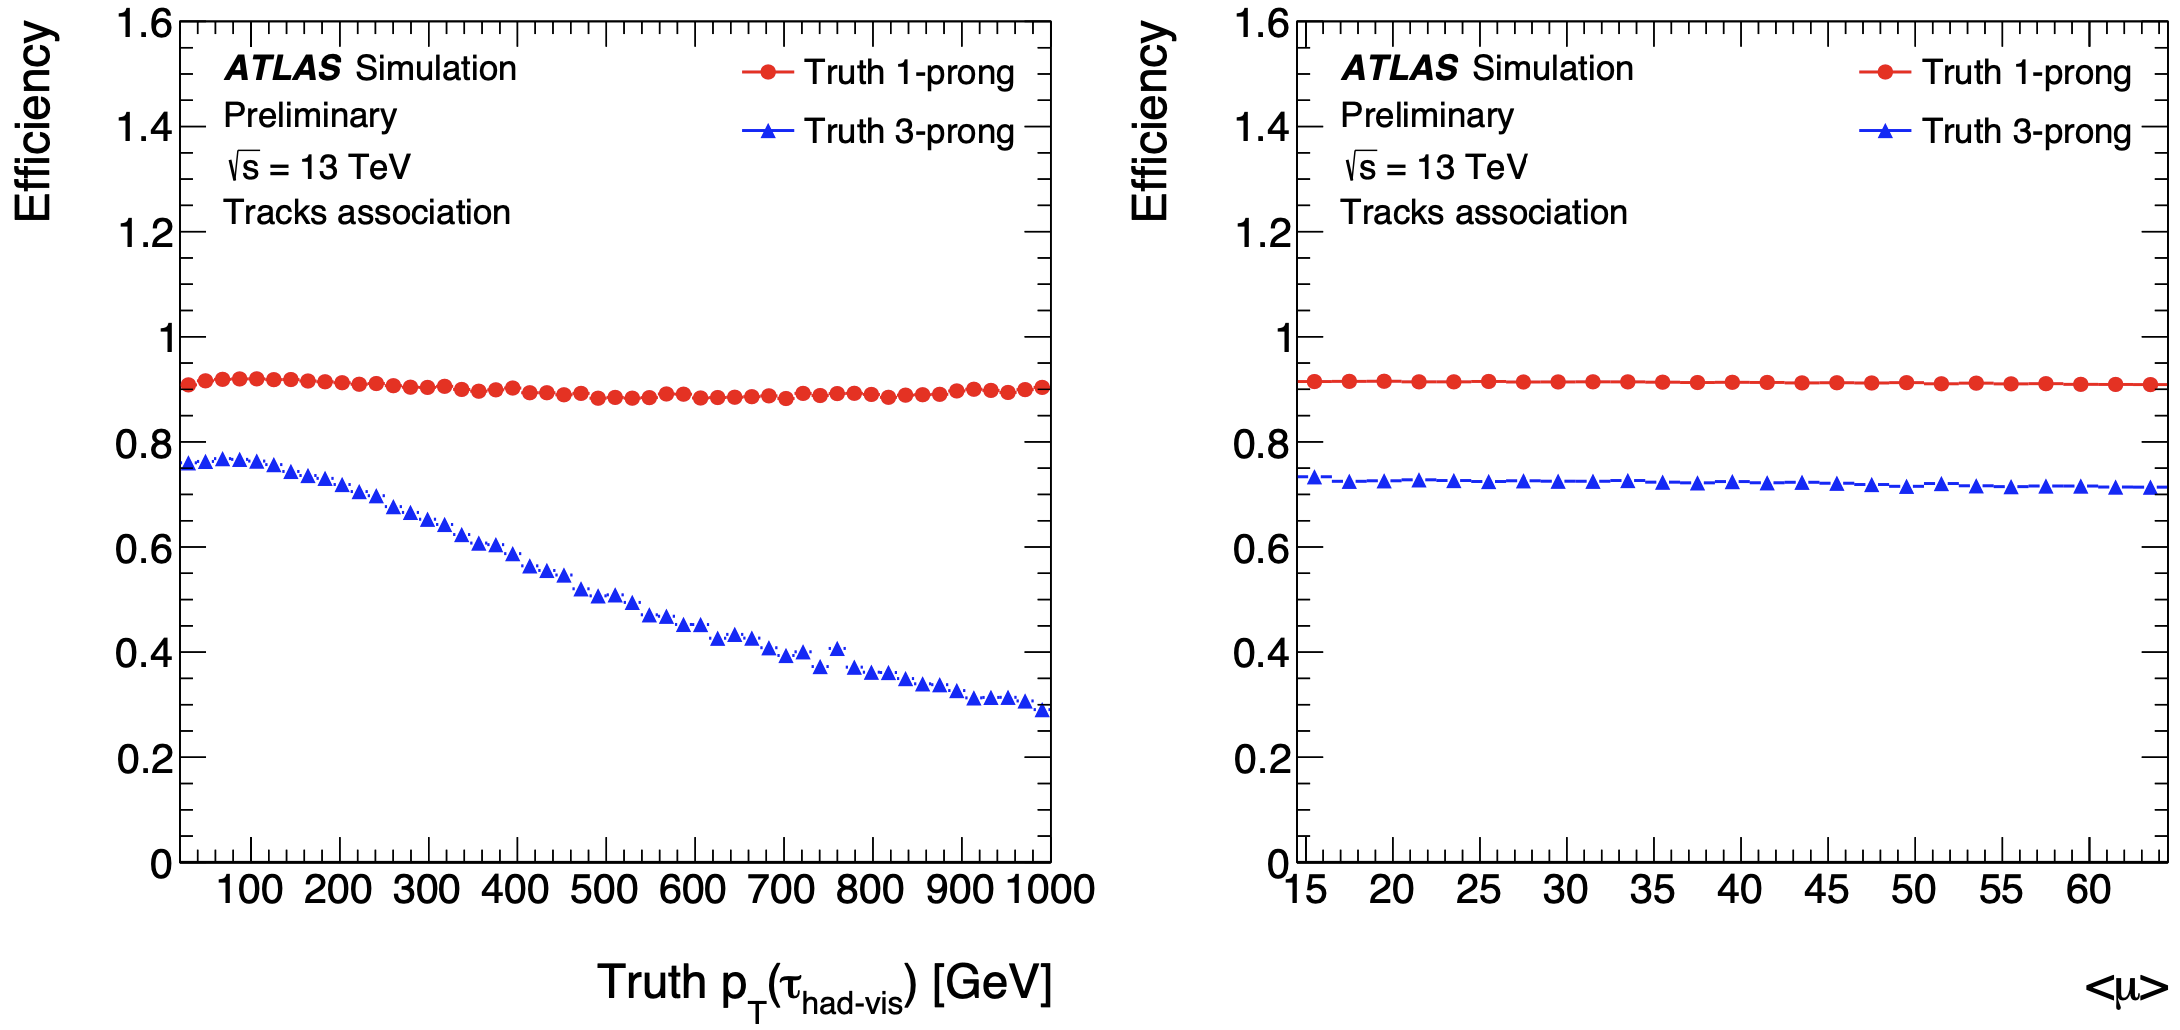
\includegraphics[width=0.9\textwidth]{taureco_eff.png}
            \caption{
                Reconstruction efficiency of the track classifier for 1-prong and 3-prong $\tauhadvis$ candidates as a function of $\tauhadvis p_T$ (left) and $\langle \mu \rangle$ (right).
            }
            \label{fig:track_classification_eff}
        \end{figure}
\section{$\tauhadvis$ Identification and electron-veto}
    \subsection{RNN-based identification}
        During Run 2, a novel $\tauhadvis$ identification algorithm (TauID)
        was introduced to separate true $\tauhadvis$ candidates 
        from those misidentified as originating from quark- and gluon-initiated 
        jets. This algorithm, based on a RNN, utilises information from reconstructed 
        charged-particle tracks and clusters of energy in the calorimeter associated 
        with $\tauhadvis$ candidates, along with high-level discriminating 
        variables. Compared to the BDT identification algorithm used at the 
        beginning of Run 2, the RNN algorithm improved the rejection of 
        misidentified $\tauhadvis$ candidates by 75-100\%, 
        depending on the $\tauhadvis$\pt and the number of tracks.

        The RNN architecture used for $\tauhadvis$ identification consists of three input branches.
        \begin{itemize}
            \item Track Variables: this branch processes information related to the tracks associated with the $\tauhadvis$candidate.
            \item Cluster Variables: this branch processes information related to the energy clusters in the calorimeter.
            \item High-Level Jet Variables: this branch processes high-level observables calculated from track and calorimeter quantities.
        \end{itemize}
        The RNN's internal state allows it to process sequences of unknown length, making it suitable for the variable-length
        input data associated with $\tauhadvis$ candidates. 
        Each branch feeds into the RNN, which is trained using simulated samples of $\tauhadvis$ candidates. 
        The signal sample consists of $\tauhadvis$ candidates from \(\gamma^* \rightarrow \tau\tau\) events,
        while the background sample consists of candidates from simulated QCD di-jet events.
        Reconstructed $\tauhadvis$ candidates from \(\gamma^* \rightarrow \tau\tau\) events are required to 
        be geometrically matched to $\tauhadvis$ at the truth level and correctly reconstructed as 1- or 3-prong decays. 
        Reconstructed $\tauhadvis$ candidates from simulated di-jet samples are required to be reconstructed as 1- or 
        3-prong $\tauhadvis$ candidates.

        The performance of the RNN-based $\tauhadvis$ identification algorithm is evaluated on independent 
        test samples of signal and background events. The efficiency of $\tauhadvis$ identification is 
        measured as a function of \tauhadvis \pT and $\langle \mu \rangle$.

        The identification algorithm defines several working points (Very Loose, Loose, Medium, Tight) based on the 
        transformed (flattened) RNN score, which ensures that the $\tauhad$ efficiency does not depend 
        on the reconstructed \tauhadvis \pT and \(\langle \mu \rangle\). The rejection of misidentified 
        $\tauhadvis$ candidates, defined as the inverse of the background selection efficiency, is evaluated 
        for each working point. The combined reconstruction and identification efficiency of the $\tauhadvis$
        identification algorithm is shown in Figure \ref{fig:tau_id_eff}. 
        Inverse of the efficiency (rejection) for misidentified 1-prong and 3-prong $\tauhad$ candidates from dijet
        background events as a function of the efficiency for truth $\tauhad$ originating from $\gamma^*\rightarrow\tau\tau$ 
        events is shown in Figure~\ref{fig:tau_id_roc}. 
        Both figures are taken from~\cite{ATL-PHYS-PUB-2022-044}.
        \begin{figure}[htbp]
            \centering
            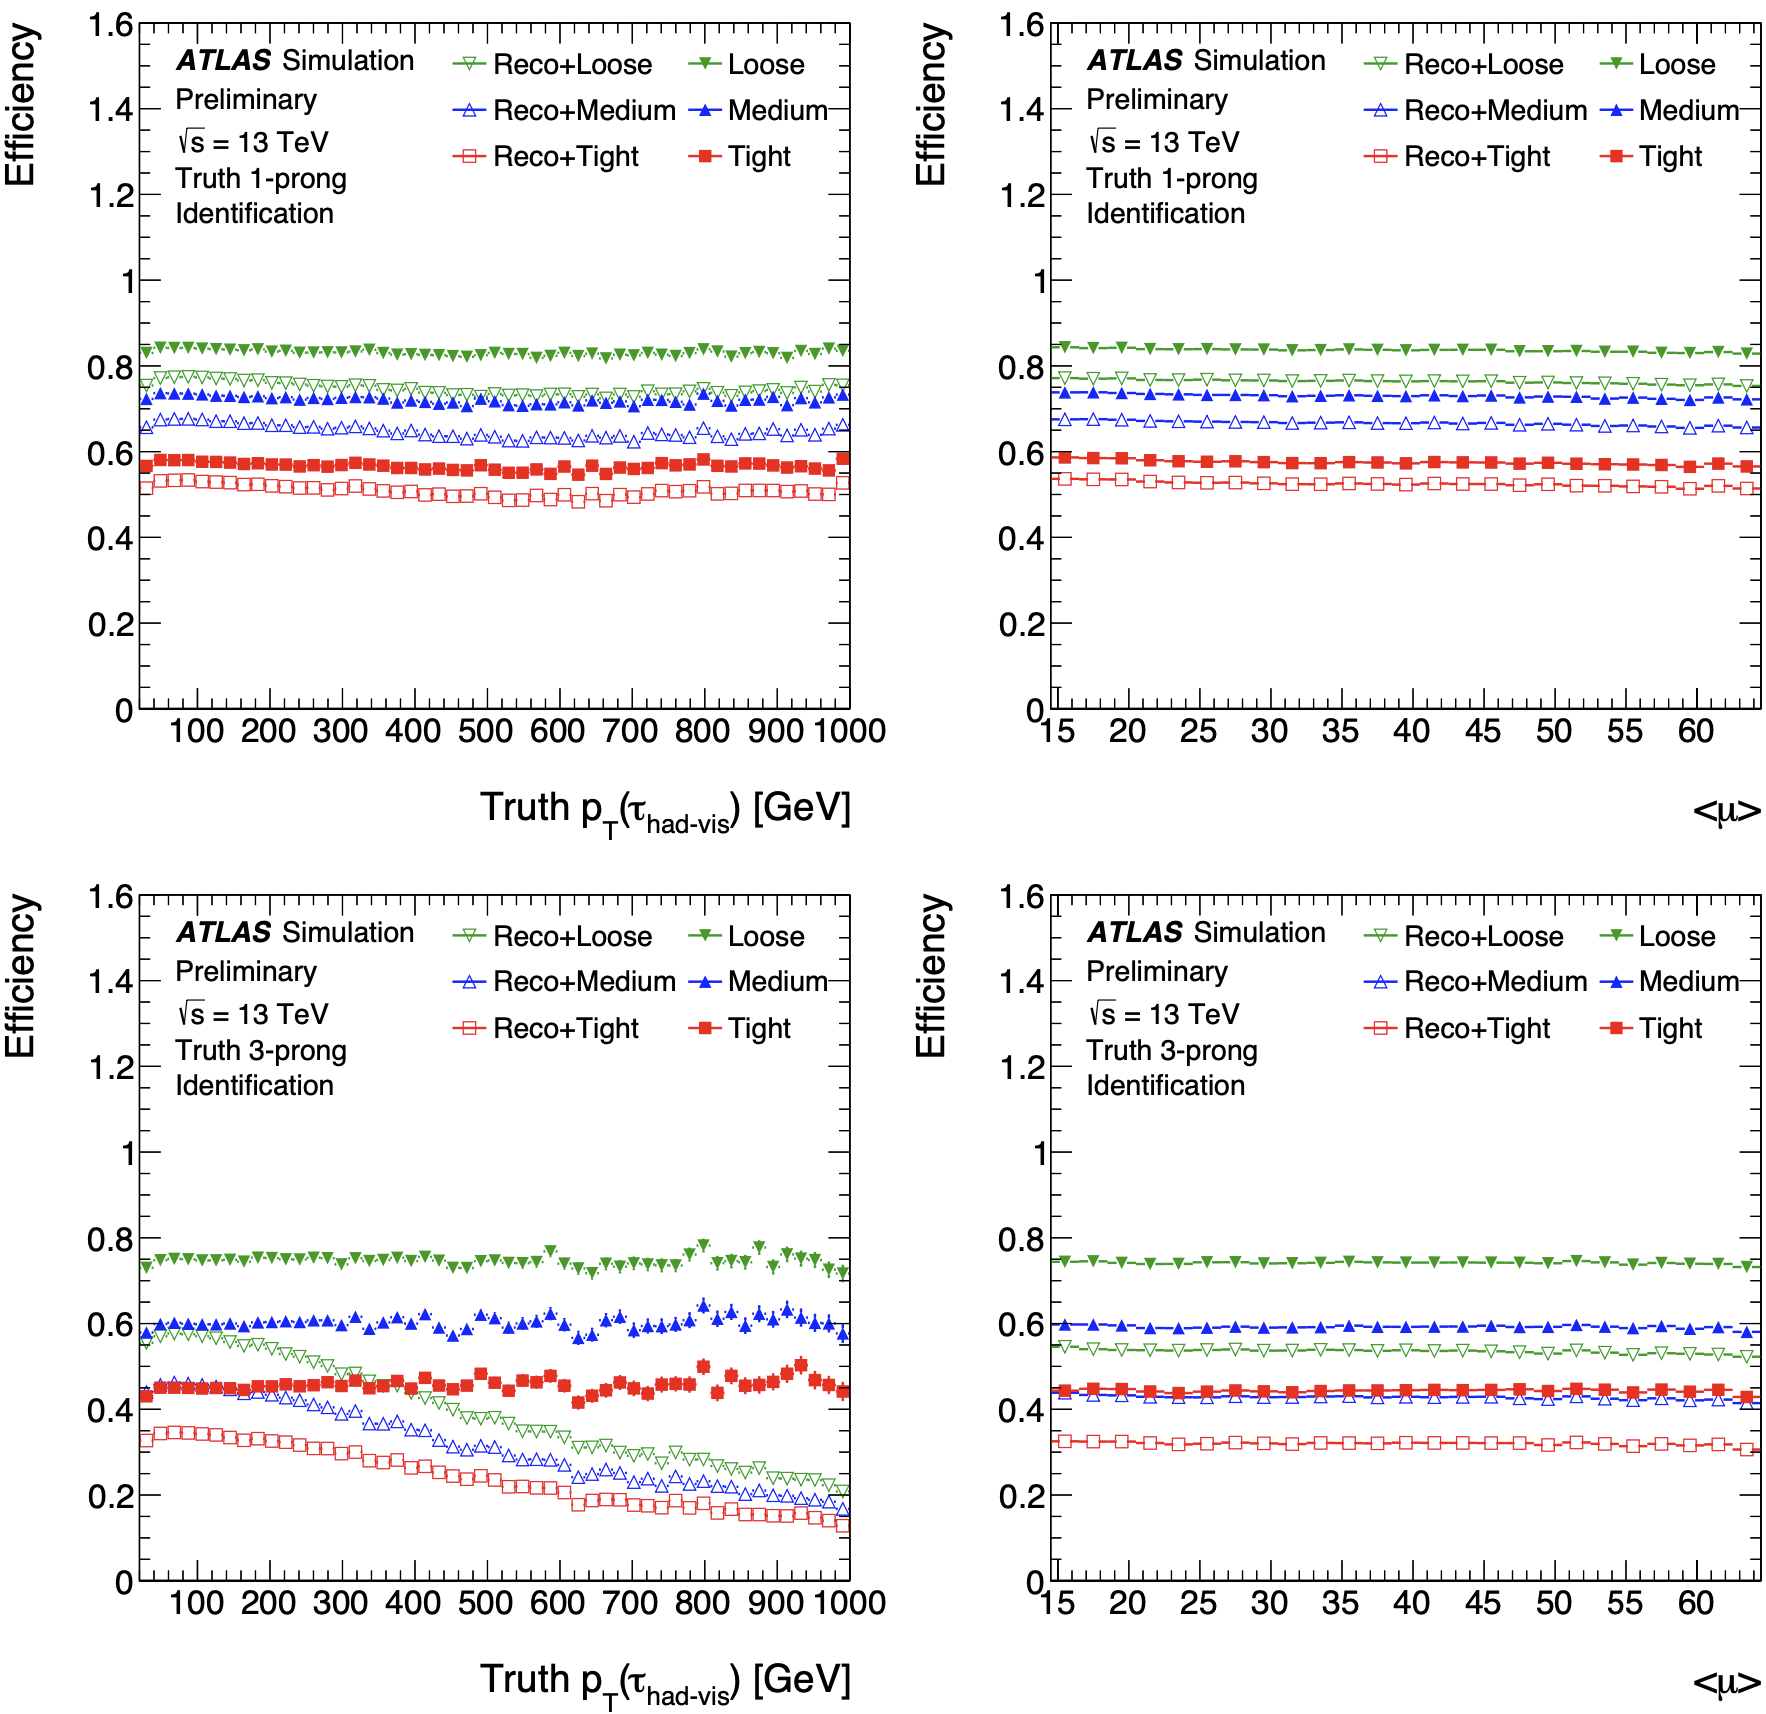
\includegraphics[width=0.9\textwidth]{tauID_eff.png}
            \caption{
                Combined reconstruction and identification efficiency of the $\tauhadvis$ identification algorithm as a 
                function of $\tauhadvis p_T$ (left) and $\langle \mu \rangle$ (right), taken from~\cite{ATL-PHYS-PUB-2022-044}.
                The decay of the $\tauhadvis$ efficiency in 3-prong $\tauhadvis$ candidates at high $\tauhadvis p_T$ is due to the
                tracking efficiency in dense environments.
            }
            \label{fig:tau_id_eff}
        \end{figure}
        \begin{figure}[htbp]
            \centering
            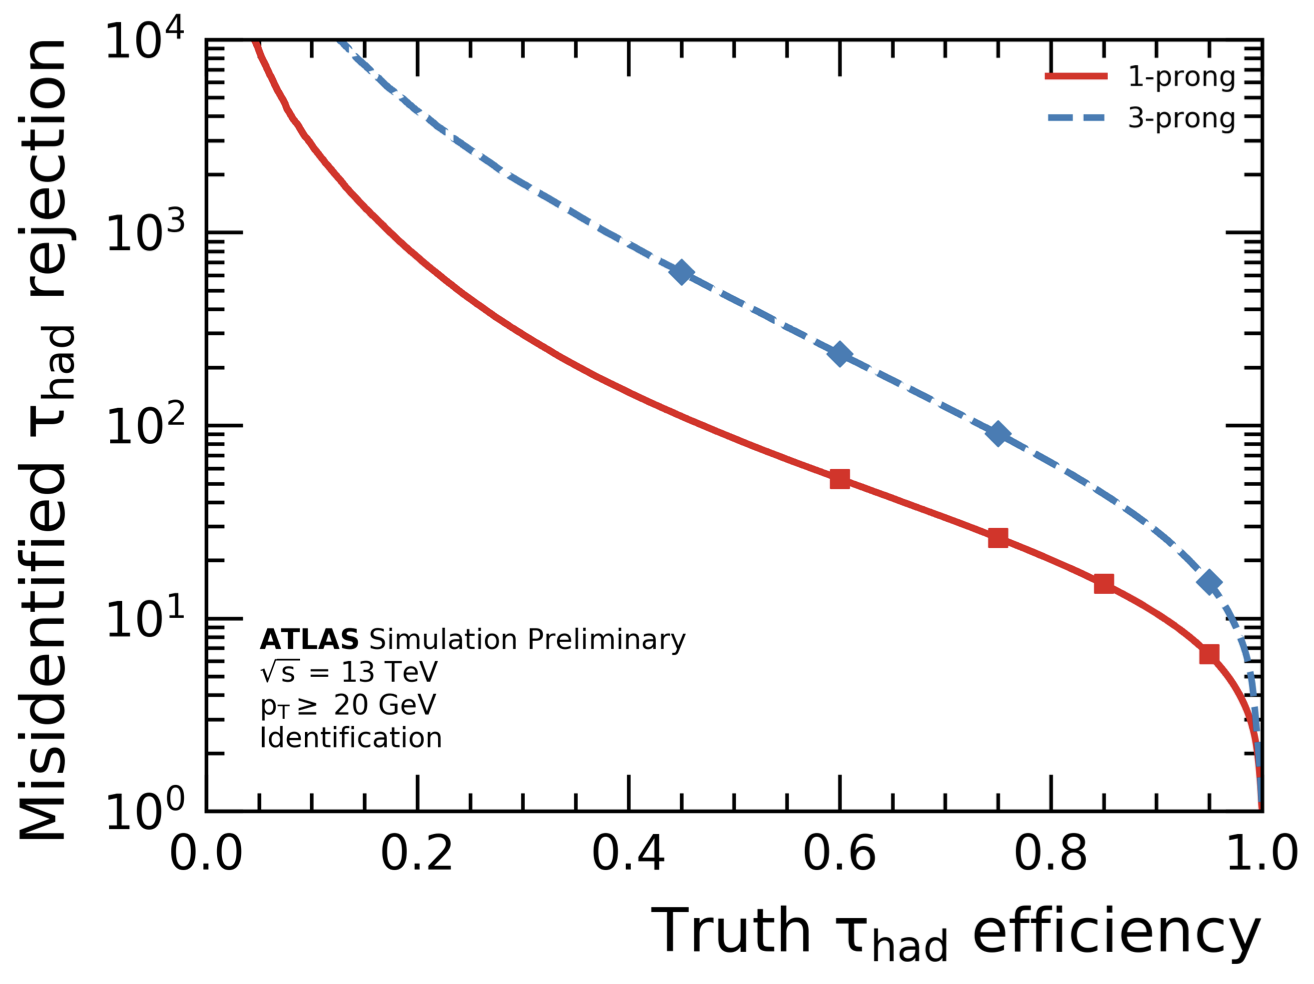
\includegraphics[width=0.45\textwidth]{tauid_roc.png}
            \caption{
                Inverse of the efficiency (rejection) for misidentified 1-prong and 3-prong $\tauhad$ candidates from dijet
                background events as a function of the efficiency for truth $\tauhad$ originating from $\gamma^*\rightarrow\tau\tau$ events, 
                taken from~\cite{ATL-PHYS-PUB-2022-044}.
            }
            \label{fig:tau_id_roc}
        \end{figure}

        The $\tauhad$ candidates are further classified into five primary decay modes by a DeepSet Neural Network (DSNN)~\cite{zaheer2018deepsets} algorithm.
        This method identifies the number of charged and neutral hadrons from $\tau$ decays. The efficiency matrix for reconstructing the same $\tau$ 
        lepton decay mode as the truth decay mode with DeepSet NN classifier in $\gamma^*\rightarrow\tau\tau$ events is shown in Figure \ref{fig:tau_decay_mode_eff}.
        \begin{figure}[htbp]
            \centering
            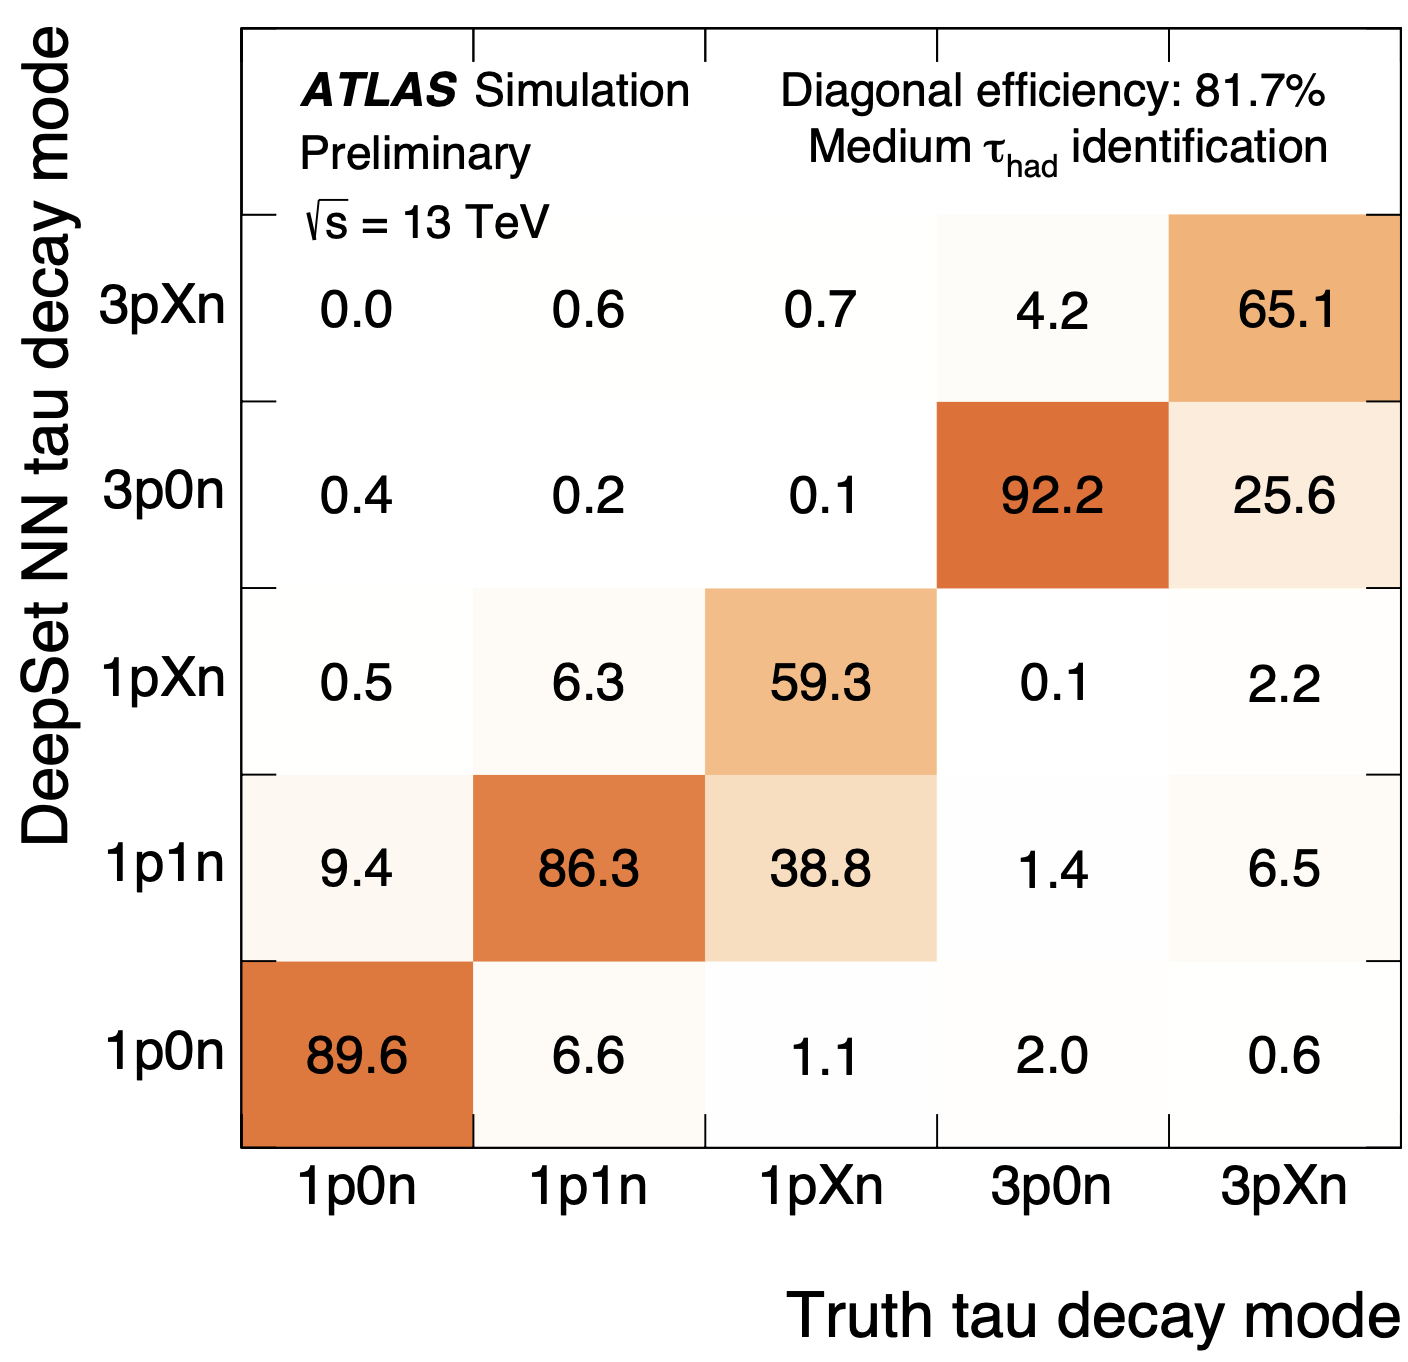
\includegraphics[width=0.45\textwidth]{decaymode_effi.png}
            \caption{
                Efficiency matrix for reconstructing the same $\tau$ lepton decay mode as the truth decay mode with DeepSet NN classifier 
                in $\gamma^*\rightarrow\tau\tau$ events, taken from~\cite{ATL-PHYS-PUB-2022-044}.
                The labels are in a form of `ApBn', where `A',`B' are the number of prongs (the `p') 
                and neutral pions (the `n') and `X' stands for more than one or more than zero accordingly.
            }
            \label{fig:tau_decay_mode_eff}
        \end{figure}

    \subsection{RNN-based electron-veto}
        Electrons can be misidentified as $\tauhadvis$ candidates. In some analyses, 
        electrons represent a significant background contribution even after the suppression of jet-related 
        backgrounds through kinematic, topological, and tau identification criteria. Despite the similarities 
        between electron signatures and 1-prong \(\tauhadvis\), there are distinctive properties 
        that can be exploited for discrimination.
        Electrons are highly relativistic particles that emit transition radiation when traversing the 
        radiator material surrounding the straws of the TRT detector. This property, along with the 
        shape of the calorimetric energy deposits in combination with the track information, provides 
        a basis for discriminating electrons from \(\tauhadvis\). The ATLAS overlap removal procedure
        ensures that identified electrons are not double-counted as $\tauhadvis$ candidates. However
        the electron identification is not perfect, and some electrons may fail the electron identification and
        still be misidentified as $\tauhadvis$.

        The BDT-based e-veto algorithm used during Run 2 has been replaced by a novel approach based on RNN. 
        The updated RNN e-veto  offers multiple 
        working points for different levels of discrimination.
        The e-veto algorithm is trained using simulated samples of signal and background candidates. The signal sample is 
        the same as that used for the TauID algorithm, while the background sample consists of reconstructed
        $\tauhadvis$ candidates from \(Z \rightarrow ee\) processes, required to pass the Medium 
        $\tauhadvis$ identification working point.
    
        Dedicated neural networks are trained separately for 1-prong and 3-prong $\tauhadvis$ cases. 
        The reconstructed \pT of the $\tauhadvis$ is used to re-weight the samples, ensuring 
        no \pT-dependent bias in the trained classifier. The training minimises the binary cross-entropy 
        loss function~\cite{mao2023crossentropylossfunctionstheoretical} using stochastic gradient descent (SGD)~\cite{ruder2016overview}
        with momentum and a step-wise reduction of the optimiser's learning rate.
    
        The e-veto algorithm's output score is transformed to provide a uniform efficiency with respect 
        to \pt and \(\eta\) of the true \(\tauhadvis\). The algorithm defines three working 
        points (Loose, Medium, Tight) for different levels of electron rejection efficiency.
        The performance of the e-veto algorithm is evaluated on independent test samples, measuring the 
        $\tauhadvis$ efficiency and electron rejection factor as functions of $\langle \mu \rangle$ and the \pt of 
        1-prong and 3-prong $\tauhadvis$ candidates.
        Figure \ref{fig:eveto_eff} shows the rejection for misidentified 1-prong and 3-prong $\tauhadvis$ candidates from $Z\rightarrow ee$
        background events as a function of the efficiency for truth $\tauhad$ originating from $\gamma^*\rightarrow\tau\tau$ events.
        \begin{figure}[htbp]
            \centering
            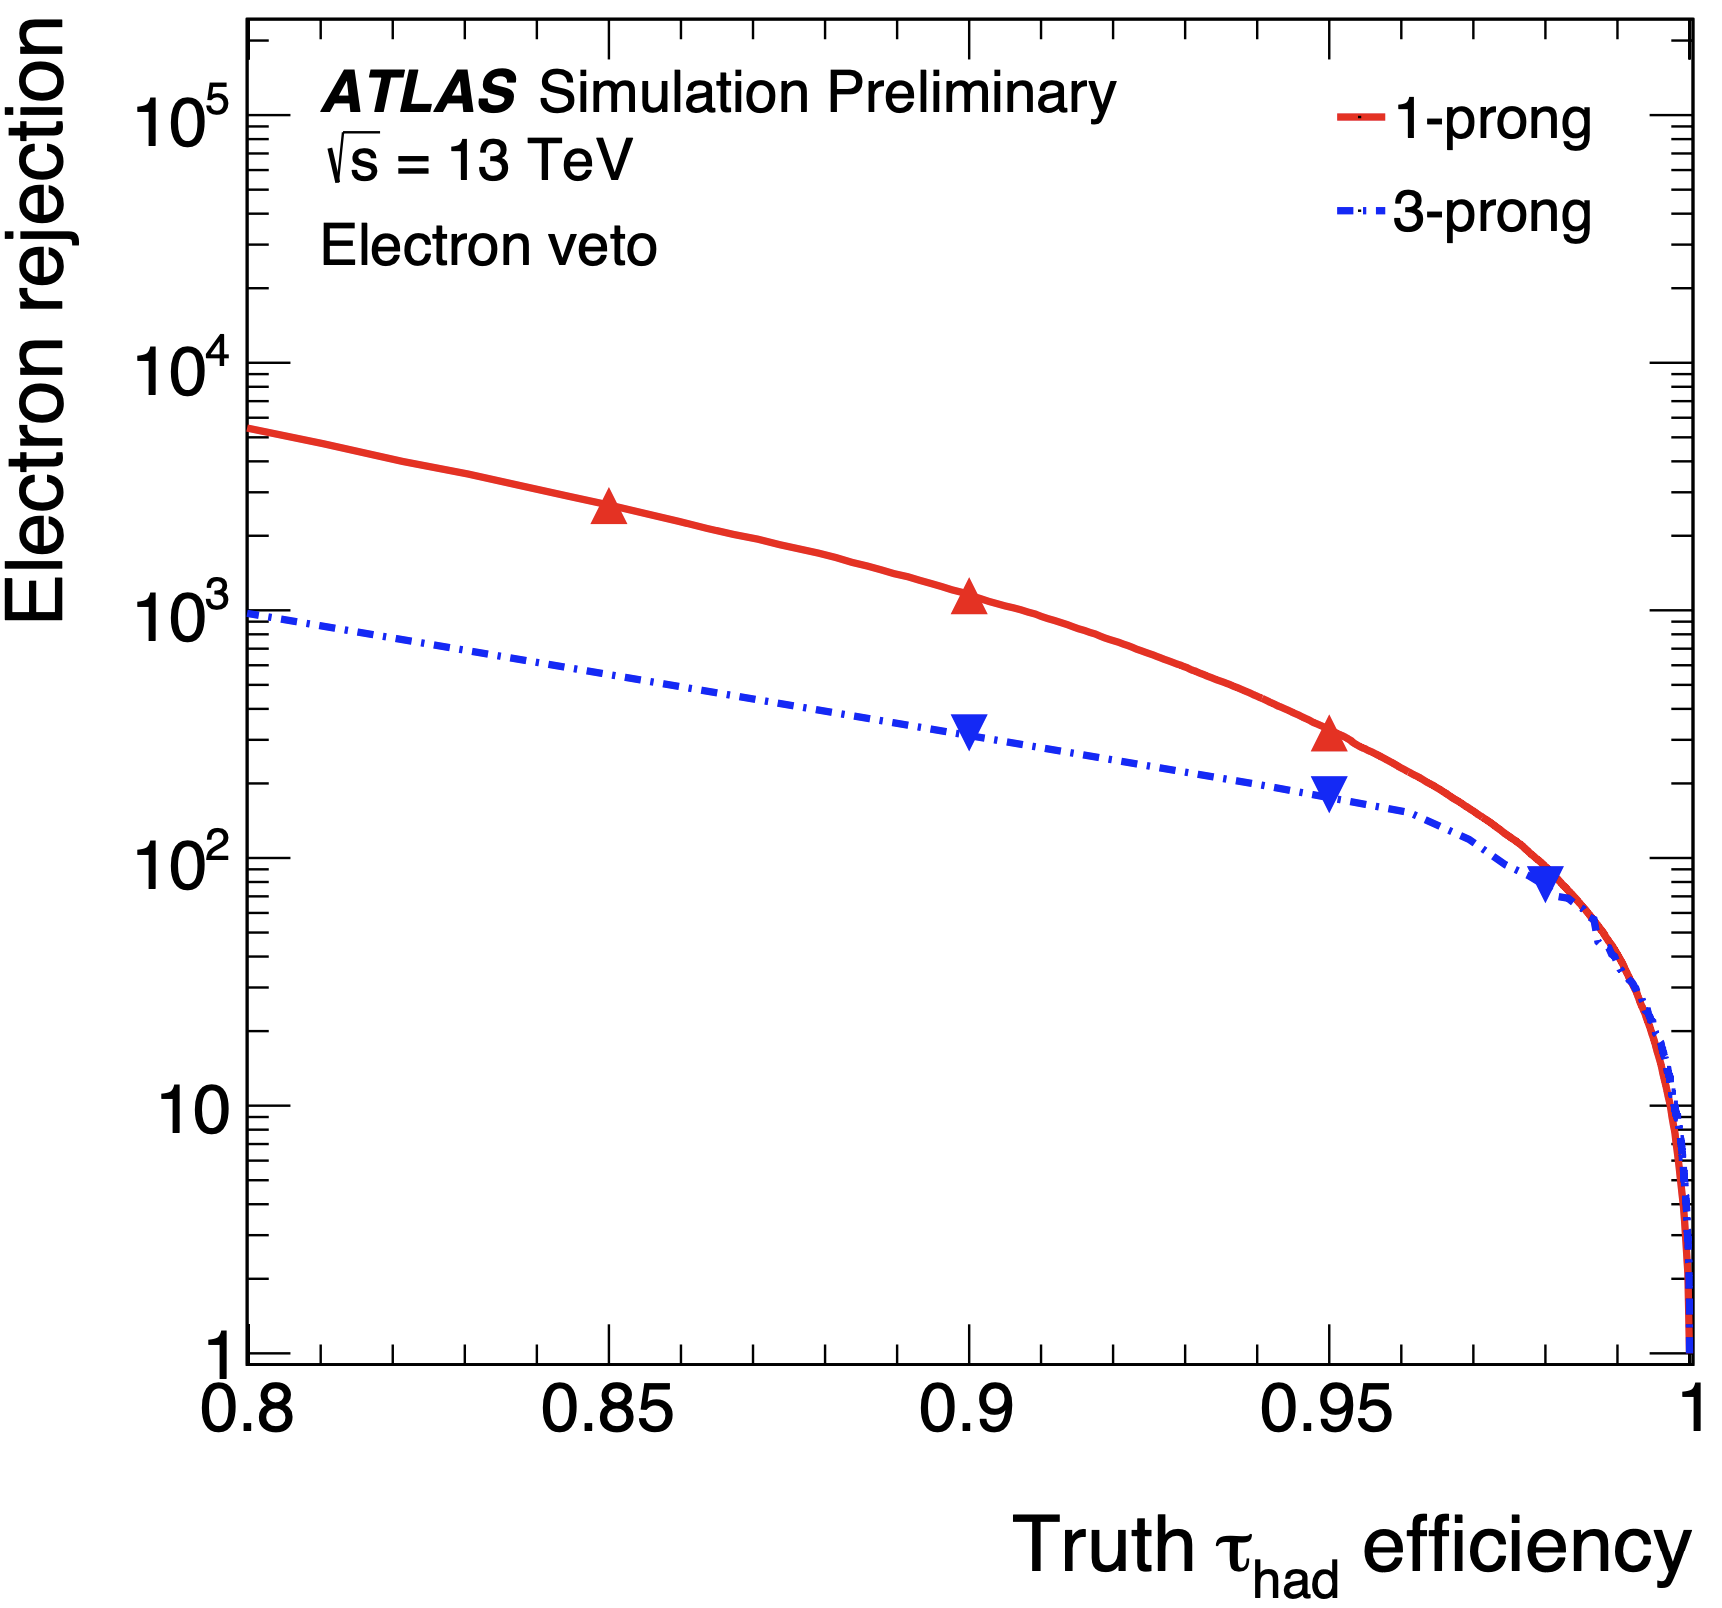
\includegraphics[width=0.45\textwidth]{eveto_roc.png}
            \caption{
                Rejection for misidentified 1-prong and 3-prong $\tauhadvis$ candidates from $Z\rightarrow ee$
                background events with the e-veto algorithm,
                as a function of the efficiency for truth $\tauhad$ originating from $\gamma^*\rightarrow\tau\tau$ events, taken from~\cite{ATL-PHYS-PUB-2022-044}.
            }
            \label{fig:eveto_eff}
        \end{figure}

\section{$\tauhadvis$ Energy calibration and resolution}
    The energy calibration of $\tauhad$ involves several steps to ensure accurate 
    measurement of the visible energy.
    \begin{itemize}
        \item Pre-calibration: initial energy estimates are obtained from the seed jets.
        \item MC-based corrections: corrections derived from MC simulations are applied to account for detector response and other systematic effects.
        \item Boosted regression tree (BRT) refinement: the boosted regression tree algorithm refines the energy estimates using additional input variables and sequential data from the RNNs.
        \item Data-driven corrections: final adjustments are made using data-driven techniques, comparing MC predictions with actual data to ensure consistency and accuracy.
    \end{itemize}

    \subsubsection{Pre-calibration}
        Pre-calibration is the initial step in the energy calibration process for $\tauhadvis$. 
        This step involves obtaining preliminary energy estimates from the visible decay products of the 
        tau leptons, utilising data from the calorimeter and tracking systems of the detector. After the 
        reconstruction of $\tauhadvis$ candidates, the four-momentum of the $\tauhadvis$
        candidate is calculated by summing the momenta of all associated clusters and tracks. 
        This preliminary four-momentum estimate provides the initial energy scale for the tau candidates.

    \subsubsection{MC-based corrections}
        The MC-based corrections are derived from detailed simulations that model the interactions of 
        particles within the detector, accounting for various physical processes and detector effects. 
        The goal of MC-based corrections is to adjust the initial energy estimates obtained during 
        pre-calibration to more accurately reflect the true energy of the tau leptons.
        
        The energy scale correction adjusts the measured energy to account for systematic biases in the 
        calorimeter and tracking systems. This ensures that the average measured energy matches the true 
        energy over a wide range of tau energies. The resolution correction accounts for the smearing of 
        the energy measurement due to detector resolution effects. It ensures that the distribution of 
        measured energies around the true energy is correctly modelled.
        
        The MC-based corrections are derived by comparing the true energy of tau leptons in the simulation
        with the energy measured by the detector. This comparison is done as a function of key variables
        like $\pT$, $|\eta|$, and decay mode. The derived correction factors are applied to the initial 
        energy estimates of $\tauhad$ candidates. The corrected energy measurements are validated 
        by comparing key distributions (e.g., invariant mass of tau pairs) in data and simulation.

    \subsubsection{BRT refinement}
        BRT refinement is a sophisticated technique used to enhance the accuracy and precision of the 
        energy estimates of $\tauhad$. This method applies machine learning to correct residual 
        biases and improve the resolution of the energy measurements beyond what is achieved by MC-based 
        corrections alone.

        At the core of BRT are decision trees, which are simple predictive models that split data into 
        subsets based on feature values. Each split is chosen to minimise the error in predicting the 
        target variable, in this case, the tau energy. Boosting is an ensemble technique that combines 
        the predictions of multiple weak learners (individual decision trees) to form a stronger predictive 
        model. Trees are built sequentially, with each tree correcting the errors of its predecessors.
    
        The energy estimates obtained from pre-calibration and MC-based corrections
        serve as the starting point for BRT refinement. The BRT model is trained using the simulated 
        samples, where the input features (calorimeter and tracking variables) are used to predict 
        the true tau energy. The model learns to correct systematic biases and improve the precision 
        of the energy estimates. Once trained, the BRT model is applied to the actual data. The model 
        takes the MC-based energy estimates and the same set of input features to produce refined 
        energy predictions for $\tauhadvis$ candidates. The performance of the BRT refinement 
        is validated using independent test samples. Key metrics such as the energy resolution and 
        scale are evaluated to ensure the model's predictions are accurate and unbiased.

    \subsubsection{Data-driven corrections}
        The data-driven method is the final step in the calibration process for $\tauhad$. 
        It involves using actual collision data to further refine and validate the energy calibration 
        obtained from MC-based corrections and BRT refinement. This approach helps to correct any 
        discrepancies between simulation and real data, ensuring that the final energy measurements 
        are as accurate and unbiased as possible~\cite{ATLAS-CONF-2017-029}.

        The data-driven method relies on reference processes to calibrate the
        energy measurements of $\tauhadvis$ candidates. Reference processes, such as
        well-understood physics decays like $\Zttmuhad$ are used as benchmarks to compare data and simulation. 
        The method exploits the fact that the distribution of the reconstructed visible mass of the $\tauhadvis$ and muon system, $m_\mathrm{vis}$, 
        in $\Zttmuhad$ events is sensitive to the differences in energy scale of the $\tauhadvis$ candidates between data and simulation.

        The $\tau$ energy scale (TES) correction is parameterised as $\pt\rightarrow(1+\alpha)\pt$ for $\tauhadvis$ candidates, where $\alpha$ is the TES correction factor.
        The muon energy scale is measured with high precision with independent methods. In Run 2, the TES correction factor is determined
        by minimising the difference between the $m_\mathrm{vis}$ distribution in data and simulation. Specifically, $\alpha$ is determined by minimising 
        $$\chi^2(\alpha, f) = \sum_i\frac{(N_i^\mathrm{data} - fN_i^\mathrm{sig}(\alpha) - N_i^\mathrm{bkg})^2}{N_i^\mathrm{data} + f^2(\Delta N_i^\mathrm{sig}(\alpha))^2+(\Delta N_i^\mathrm{bkg})^2},$$
        where $N_i^\mathrm{data/sig/bkg}$ is the number of events in the $i$-th bin of the $m_\mathrm{vis}$ distribution in data, signal, or background; 
        $\Delta N_i^\mathrm{sig}$ is the uncertainty in the number of signal events in the $i$-th bin; 
        and $f$ is a normalisation factor that accounts for the difference in the total number of events between data and simulation.
        